
%% bare_conf.tex
%% V1.3
%% 2007/01/11
%% by Michael Shell
%% See:
%% http://www.michaelshell.org/
%% for current contact information.
%%
%% This is a skeleton file demonstrating the use of IEEEtran.cls
%% (requires IEEEtran.cls version 1.7 or later) with an IEEE conference paper.
%%
%% Support sites:
%% http://www.michaelshell.org/tex/ieeetran/
%% http://www.ctan.org/tex-archive/macros/latex/contrib/IEEEtran/
%% and
%% http://www.ieee.org/

%%*************************************************************************
%% Legal Notice:
%% This code is offered as-is without any warranty either expressed or
%% implied; without even the implied warranty of MERCHANTABILITY or
%% FITNESS FOR A PARTICULAR PURPOSE!
%% User assumes all risk.
%% In no event shall IEEE or any contributor to this code be liable for
%% any damages or losses, including, but not limited to, incidental,
%% consequential, or any other damages, resulting from the use or misuse
%% of any information contained here.
%%
%% All comments are the opinions of their respective authors and are not
%% necessarily endorsed by the IEEE.
%%
%% This work is distributed under the LaTeX Project Public License (LPPL)
%% ( http://www.latex-project.org/ ) version 1.3, and may be freely used,
%% distributed and modified. A copy of the LPPL, version 1.3, is included
%% in the base LaTeX documentation of all distributions of LaTeX released
%% 2003/12/01 or later.
%% Retain all contribution notices and credits.
%% ** Modified files should be clearly indicated as such, including  **
%% ** renaming them and changing author support contact information. **
%%
%% File list of work: IEEEtran.cls, IEEEtran_HOWTO.pdf, bare_adv.tex,
%%                    bare_conf.tex, bare_jrnl.tex, bare_jrnl_compsoc.tex
%%*************************************************************************

% *** Authors should verify (and, if needed, correct) their LaTeX system  ***
% *** with the testflow diagnostic prior to trusting their LaTeX platform ***
% *** with production work. IEEE's font choices can trigger bugs that do  ***
% *** not appear when using other class files.                            ***
% The testflow support page is at:
% http://www.michaelshell.org/tex/testflow/



% Note that the a4paper option is mainly intended so that authors in
% countries using A4 can easily print to A4 and see how their papers will
% look in print - the typesetting of the document will not typically be
% affected with changes in paper size (but the bottom and side margins will).
% Use the testflow package mentioned above to verify correct handling of
% both paper sizes by the user's LaTeX system.
%
% Also note that the "draftcls" or "draftclsnofoot", not "draft", option
% should be used if it is desired that the figures are to be displayed in
% draft mode.
%
\documentclass[conference]{IEEEtran}
% Add the compsoc option for Computer Society conferences.
%
% If IEEEtran.cls has not been installed into the LaTeX system files,
% manually specify the path to it like:
% \documentclass[conference]{../sty/IEEEtran}





% Some very useful LaTeX packages include:
% (uncomment the ones you want to load)


% *** MISC UTILITY PACKAGES ***
%
%\usepackage{ifpdf}
% Heiko Oberdiek's ifpdf.sty is very useful if you need conditional
% compilation based on whether the output is pdf or dvi.
% usage:
% \ifpdf
%   % pdf code
% \else
%   % dvi code
% \fi
% The latest version of ifpdf.sty can be obtained from:
% http://www.ctan.org/tex-archive/macros/latex/contrib/oberdiek/
% Also, note that IEEEtran.cls V1.7 and later provides a builtin
% \ifCLASSINFOpdf conditional that works the same way.
% When switching from latex to pdflatex and vice-versa, the compiler may
% have to be run twice to clear warning/error messages.






% *** CITATION PACKAGES ***
%
%\usepackage{cite}
% cite.sty was written by Donald Arseneau
% V1.6 and later of IEEEtran pre-defines the format of the cite.sty package
% \cite{} output to follow that of IEEE. Loading the cite package will
% result in citation numbers being automatically sorted and properly
% "compressed/ranged". e.g., [1], [9], [2], [7], [5], [6] without using
% cite.sty will become [1], [2], [5]--[7], [9] using cite.sty. cite.sty's
% \cite will automatically add leading space, if needed. Use cite.sty's
% noadjust option (cite.sty V3.8 and later) if you want to turn this off.
% cite.sty is already installed on most LaTeX systems. Be sure and use
% version 4.0 (2003-05-27) and later if using hyperref.sty. cite.sty does
% not currently provide for hyperlinked citations.
% The latest version can be obtained at:
% http://www.ctan.org/tex-archive/macros/latex/contrib/cite/
% The documentation is contained in the cite.sty file itself.






% *** GRAPHICS RELATED PACKAGES ***
%
\ifCLASSINFOpdf
  % \usepackage[pdftex]{graphicx}
  % declare the path(s) where your graphic files are
  % \graphicspath{{../pdf/}{../jpeg/}}
  % and their extensions so you won't have to specify these with
  % every instance of \includegraphics
  % \DeclareGraphicsExtensions{.pdf,.jpeg,.png}
\else
  % or other class option (dvipsone, dvipdf, if not using dvips). graphicx
  % will default to the driver specified in the system graphics.cfg if no
  % driver is specified.
   \usepackage[dvips]{graphicx}
  % declare the path(s) where your graphic files are
  % \graphicspath{{../eps/}}
  % and their extensions so you won't have to specify these with
  % every instance of \includegraphics
  % \DeclareGraphicsExtensions{.eps}
\fi
% graphicx was written by David Carlisle and Sebastian Rahtz. It is
% required if you want graphics, photos, etc. graphicx.sty is already
% installed on most LaTeX systems. The latest version and documentation can
% be obtained at:
% http://www.ctan.org/tex-archive/macros/latex/required/graphics/
% Another good source of documentation is "Using Imported Graphics in
% LaTeX2e" by Keith Reckdahl which can be found as epslatex.ps or
% epslatex.pdf at: http://www.ctan.org/tex-archive/info/
%
% latex, and pdflatex in dvi mode, support graphics in encapsulated
% postscript (.eps) format. pdflatex in pdf mode supports graphics
% in .pdf, .jpeg, .png and .mps (metapost) formats. Users should ensure
% that all non-photo figures use a vector format (.eps, .pdf, .mps) and
% not a bitmapped formats (.jpeg, .png). IEEE frowns on bitmapped formats
% which can result in "jaggedy"/blurry rendering of lines and letters as
% well as large increases in file sizes.
%
% You can find documentation about the pdfTeX application at:
% http://www.tug.org/applications/pdftex





% *** MATH PACKAGES ***
%
%\usepackage[cmex10]{amsmath}
% A popular package from the American Mathematical Society that provides
% many useful and powerful commands for dealing with mathematics. If using
% it, be sure to load this package with the cmex10 option to ensure that
% only type 1 fonts will utilized at all point sizes. Without this option,
% it is possible that some math symbols, particularly those within
% footnotes, will be rendered in bitmap form which will result in a
% document that can not be IEEE Xplore compliant!
%
% Also, note that the amsmath package sets \interdisplaylinepenalty to 10000
% thus preventing page breaks from occurring within multiline equations. Use:
%\intisplaylinepenalty=2500 erd
% after loading amsmath to restore such page breaks as IEEEtran.cls normally
% does. amsmath.sty is already installed on most LaTeX systems. The latest
% version and documentation can be obtained at:
% http://www.ctan.org/tex-archive/macros/latex/required/amslatex/math/





% *** SPECIALIZED LIST PACKAGES ***
%
%\usepackage{algorithmic}
% algorithmic.sty was written by Peter Williams and Rogerio Brito.
% This package provides an algorithmic environment fo describing algorithms.
% You can use the algorithmic environment in-text or within a figure
% environment to provide for a floating algorithm. Do NOT use the algorithm
% floating environment provided by algorithm.sty (by the same authors) or
% algorithm2e.sty (by Christophe Fiorio) as IEEE does not use dedicated
% algorithm float types and packages that provide these will not provide
% correct IEEE style captions. The latest version and documentation of
% algorithmic.sty can be obtained at:
% http://www.ctan.org/tex-archive/macros/latex/contrib/algorithms/
% There is also a support site at:
% http://algorithms.berlios.de/index.html
% Also of interest may be the (relatively newer and more customizable)
% algorithmicx.sty package by Szasz Janos:
% http://www.ctan.org/tex-archive/macros/latex/contrib/algorithmicx/




% *** ALIGNMENT PACKAGES ***
%
%\usepackage{array}
% Frank Mittelbach's and David Carlisle's array.sty patches and improves
% the standard LaTeX2e array and tabular environments to provide better
% appearance and additional user controls. As the default LaTeX2e table
% generation code is lacking to the point of almost being broken with
% respect to the quality of the end results, all users are strongly
% advised to use an enhanced (at the very least that provided by array.sty)
% set of table tools. array.sty is already installed on most systems. The
% latest version and documentation can be obtained at:
% http://www.ctan.org/tex-archive/macros/latex/required/tools/


%\usepackage{mdwmath}
%\usepackage{mdwtab}
% Also highly recommended is Mark Wooding's extremely powerful MDW tools,
% especially mdwmath.sty and mdwtab.sty which are used to format equations
% and tables, respectively. The MDWtools set is already installed on most
% LaTeX systems. The lastest version and documentation is available at:
% http://www.ctan.org/tex-archive/macros/latex/contrib/mdwtools/


% IEEEtran contains the IEEEeqnarray family of commands that can be used to
% generate multiline equations as well as matrices, tables, etc., of high
% quality.


%\usepackage{eqparbox}
% Also of notable interest is Scott Pakin's eqparbox package for creating
% (automatically sized) equal width boxes - aka "natural width parboxes".
% Available at:
% http://www.ctan.org/tex-archive/macros/latex/contrib/eqparbox/





% *** SUBFIGURE PACKAGES ***
%\usepackage[tight,footnotesize]{subfigure}
% subfigure.sty was written by Steven Douglas Cochran. This package makes it
% easy to put subfigures in your figures. e.g., "Figure 1a and 1b". For IEEE
% work, it is a good idea to load it with the tight package option to reduce
% the amount of white space around the subfigures. subfigure.sty is already
% installed on most LaTeX systems. The latest version and documentation can
% be obtained at:
% http://www.ctan.org/tex-archive/obsolete/macros/latex/contrib/subfigure/
% subfigure.sty has been superceeded by subfig.sty.



%\usepackage[caption=false]{caption}
%\usepackage[font=footnotesize]{subfig}
% subfig.sty, also written by Steven Douglas Cochran, is the modern
% replacement for subfigure.sty. However, subfig.sty requires and
% automatically loads Axel Sommerfeldt's caption.sty which will override
% IEEEtran.cls handling of captions and this will result in nonIEEE style
% figure/table captions. To prevent this problem, be sure and preload
% caption.sty with its "caption=false" package option. This is will preserve
% IEEEtran.cls handing of captions. Version 1.3 (2005/06/28) and later
% (recommended due to many improvements over 1.2) of subfig.sty supports
% the caption=false option directly:
%\usepackage[caption=false,font=footnotesize]{subfig}
%
% The latest version and documentation can be obtained at:
% http://www.ctan.org/tex-archive/macros/latex/contrib/subfig/
% The latest version and documentation of caption.sty can be obtained at:
% http://www.ctan.org/tex-archive/macros/latex/contrib/caption/




% *** FLOAT PACKAGES ***
%
%\usepackage{fixltx2e}
% fixltx2e, the successor to the earlier fix2col.sty, was written by
% Frank Mittelbach and David Carlisle. This package corrects a few problems
% in the LaTeX2e kernel, the most notable of which is that in current
% LaTeX2e releases, the ordering of single and double column floats is not
% guaranteed to be preserved. Thus, an unpatched LaTeX2e can allow a
% single column figure to be placed prior to an earlier double column
% figure. The latest version and documentation can be found at:
% http://www.ctan.org/tex-archive/macros/latex/base/



%\usepackage{stfloats}
% stfloats.sty was written by Sigitas Tolusis. This package gives LaTeX2e
% the ability to do double column floats at the bottom of the page as well
% as the top. (e.g., "\begin{figure*}[!b]" is not normally possible in
% LaTeX2e). It also provides a command:
%\fnbelowfloat
% to enable the placement of footnotes below bottom floats (the standard
% LaTeX2e kernel puts them above bottom floats). This is an invasive package
% which rewrites many portions of the LaTeX2e float routines. It may not work
% with other packages that modify the LaTeX2e float routines. The latest
% version and documentation can be obtained at:
% http://www.ctan.org/tex-archive/macros/latex/contrib/sttools/
% Documentation is contained in the stfloats.sty comments as well as in the
% presfull.pdf file. Do not use the stfloats baselinefloat ability as IEEE
% does not allow \baselineskip to stretch. Authors submitting work to the
% IEEE should note that IEEE rarely uses double column equations and
% that authors should try to avoid such use. Do not be tempted to use the
% cuted.sty or midfloat.sty packages (also by Sigitas Tolusis) as IEEE does
% not format its papers in such ways.





% *** PDF, URL AND HYPERLINK PACKAGES ***
%
%\usepackage{url}
% url.sty was written by Donald Arseneau. It provides better support for
% handling and breaking URLs. url.sty is already installed on most LaTeX
% systems. The latest version can be obtained at:
% http://www.ctan.org/tex-archive/macros/latex/contrib/misc/
% Read the url.sty source comments for usage information. Basically,
% \url{my_url_here}.





% *** Do not adjust lengths that control margins, column widths, etc. ***
% *** Do not use packages that alter fonts (such as pslatex).         ***
% There should be no need to do such things with IEEEtran.cls V1.6 and later.
% (Unless specifically asked to do so by the journal or conference you plan
% to submit to, of course. )


% correct bad hyphenation here
\hyphenation{op-tical net-works semi-conduc-tor}
\usepackage{graphicx}
\usepackage{pdfpages}
\usepackage[cmex10]{amsmath}
\usepackage{enumerate}
\usepackage{epstopdf}
\begin{document}
%
% paper title
% can use linebreaks \\ within to get better formatting as desired
\title{A smart explicitness congestion notification transport control mechanism for NDN}


% author names and affiliations
% use a multiple column layout for up to three different
% affiliations

%\author{\IEEEauthorblockN{Michael Shell}
%\IEEEauthorblockA{School of Electrical and\\Computer Engineering\\
%Georgia Institute of Technology\\
%Atlanta, Georgia 30332--0250\\
%Email: http://www.michaelshell.org/contact.html}
%\and
%\IEEEauthorblockN{Homer Simpson}
%\IEEEauthorblockA{Twentieth Century Fox\\
%Springfield, USA\\
%Email: homer@thesimpsons.com}
%\and
%\IEEEauthorblockN{James Kirk\\ and Montgomery Scott}
%\IEEEauthorblockA{Starfleet Academy\\
%San Francisco, California 96678-2391\\
%Telephone: (800) 555--1212\\
%Fax: (888) 555--1212}}

% conference papers do not typically use \thanks and this command
% is locked out in conference mode. If really needed, such as for
% the acknowledgment of grants, issue a \IEEEoverridecommandlockouts
% after \documentclass

% for over three affiliations, or if they all won't fit within the width
% of the page, use this alternative format:
%
\author{\IEEEauthorblockN{Jianer Zhou\IEEEauthorrefmark{1}\IEEEauthorrefmark{2},
Zhenyu Li\IEEEauthorrefmark{1},
Qinghua Wu\IEEEauthorrefmark{1}\IEEEauthorrefmark{2},
Yonggong Wang\IEEEauthorrefmark{1}\IEEEauthorrefmark{2},
Gaogang Xie\IEEEauthorrefmark{1}}
\IEEEauthorblockA{\IEEEauthorrefmark{1}Institute of Computing Technology, Chinese Academy of Sciences, Beijing, China\\
\{zhoujianer, zyli, wuqinghua, wangyonggong, xieg\}@ict.ac.cn}
\IEEEauthorblockA{\IEEEauthorrefmark{2}Graduate School of Chinese Academy of Sciences, Beijing, China}}






% use for special paper notices
%\IEEEspecialpapernotice{(Invited Paper)}




% make the title area
\maketitle


\begin{abstract}
%\boldmath
Named Data Network(NDN) is a new Internet architecture. Its changes of the network layer also shed light on the transport layer. The Data coming back along the same path of the Interest natively acts as a barrier of the Explicit Congestion Notification (ECN) information to receiver.  Avoiding a congesting path can be achieved by adaptive forwarding which is a main feature of the NDN data plane. In this paper we implement an ECN transport mechanism in NDN, using the Data to carry ECN information. And we make use of network-wide information of the SDN controller  to design smart forwarding mechanism. Our simulation in ndnSim shows that the ECN transport mechanism out-performance TCP-style NDN transport mechanisms in link utilization, packet dropping and flow complete time. The network-view information of the SDN controller can optimize the adaptive forwarding in NDN. By joining the ECN congestion mechanism and smart forwarding, the total flow complete time can be reduced.

\emph{Index Terms}-NDN, Transport mechanism, ECN, Congestion control, Adaptive forwarding
\end{abstract}
% IEEEtran.cls defaults to using nonbold math in the Abstract.
% This preserves the distinction between vectors and scalars. However,
% if the conference you are submitting to favors bold math in the abstract,
% then you can use LaTeX's standard command \boldmath at the very start
% of the abstract to achieve this. Many IEEE journals/conferences frown on
% math in the abstract anyway.

% no keywords




% For peer review papers, you can put extra information on the cover
% page as needed:
% \ifCLASSOPTIONpeerreview
% \begin{center} \bfseries EDICS Category: 3-BBND \end{center}
% \fi
%
% For peerreview papers, this IEEEtran command inserts a page break and
% creates the second title. It will be ignored for other modes.
\IEEEpeerreviewmaketitle



\section{Introduction}
% no \IEEEPARstart
People now using network care more about ``what" they can get from network. However TCP/IP, the network architecture of Internet, is initially designed based on the principle of ``where" to connect the users. This mismatch between the user-demand and network-principle makes the network difficult to satisfy the users. To overcome this, some clean-state network architecture have been proposed. NDN is one of such clean-state architecture\cite{NDN}.In NDN, users just send Interest into the network, and the network will return the corresponding Data to it, unnecessary to care about where to get the Data.

As the NDN network layer is still based on the best-effort transmit model, it is necessary to use transport control to guarantee effective transfer. Some TCP-style transport control mechanisms have been proposed for NDN, such ICP\cite{ICP}, CCTCP\cite{CCTCP} and HR-ICP\cite{shape}. However these TCP-style transport mechanisms in NDN still have same problems as TCP/IP, such as low link utilization, and high packets dropping rate. Explicit congestion notification(ECN) is a promise way to achieve high link utilization\cite{XCP} . Adaptive forwarding is a new feature of the NDN\cite{Adaptive}. Adaptive forwarding let router choose a suitable path according the network situation. If the router sense the link has been congested, then it can choose another path. It is completely different with TCP/IP, as in TCP/IP the forwarding process is strictly followed the route table. By make use of the adaptive forwarding, router can deal with the network congestion quickly.

But by now, as what we have known, there is not ECN-style congestion mechanism proposed in NDN and there is little research about the congestion avoiding mechanism making use of the adaptive forwarding. In this paper we use the Data(which come back along the same way of Interest) to carry the ECN information, and design an ECN transport mechanism for NDN. We also make use of the SDN's network-wide information to choose a suitable forwarding interface\cite{SDN}. Joining the ECN and smart-adaptive forwarding mechanism, we can not only improve single link bandwidth utilization but also the whole network resource utilization. Summary, our main contributions are:
\begin{enumerate}
\item[1.]First achieve an ECN transport mechanism in NDN.

\item[2.]First use SDN-style control information to design smart forwarding mechanism to ultimately use the whole network resource.

\item[3.] Packet-level simulation shows that joining ECN and smart forwarding in NDN can improve link utilization and the total flow complete time.
\end{enumerate}
The rest of the paper is organized as followed: in Sec. \uppercase\expandafter{\romannumeral 2} we will introduce the NDN's feature that we will use to design our transport mechanism. In Sec. \uppercase\expandafter{\romannumeral 3} we will discuss the design rationale. In Sec. \uppercase\expandafter{\romannumeral 4} we will introduce the ECN congestion mechanism and the SDN-style smart forwarding. In Sec. \uppercase\expandafter{\romannumeral 5}, we demonstrate the effectiveness of our mechanism. In Sec. \uppercase\expandafter{\romannumeral 6}, we will introduce related work. Finally Sec. \uppercase\expandafter{\romannumeral 7} concludes the paper.


% You must have at least 2 lines in the paragraph with the drop letter
% (should never be an issue)


%\subsection{Subsection Heading Here}
%Subsection text here.


%\subsubsection{Subsubsection Heading Here}
%Subsubsection text here.


% An example of a floating figure using the graphicx package.
% Note that \label must occur AFTER (or within) \caption.
% For figures, \caption should occur after the \includegraphics.
% Note that IEEEtran v1.7 and later has special internal code that
% is designed to preserve the operation of \label within \caption
% even when the captionsoff option is in effect. However, because
% of issues like this, it may be the safest practice to put all your
% \label just after \caption rather than within \caption{}.
%
% Reminder: the "draftcls" or "draftclsnofoot", not "draft", class
% option should be used if it is desired that the figures are to be
% displayed while in draft mode.
%
%\begin{figure}[!t]
%\centering
%\includegraphics[width=2.5in]{myfigure}
% where an .eps filename suffix will be assumed under latex,
% and a .pdf suffix will be assumed for pdflatex; or what has been declared
% via \DeclareGraphicsExtensions.
%\caption{Simulation Results}
%\label{fig_sim}
%\end{figure}


% Note that IEEE typically puts floats only at the top, even when this
% results in a large percentage of a column being occupied by floats.


% An example of a double column floating figure using two subfigures.
% (The subfig.sty package must be loaded for this to work.)
% The subfigure \label commands are set within each subfloat command, the
% \label for the overall figure must come after \caption.
% \hfil must be used as a separator to get equal spacing.
% The subfigure.sty package works much the same way, except \subfigure is
% used instead of \subfloat.
%
%\begin{figure*}[!t]
%\centerline{\subfloat[Case I]\includegraphics[width=2.5in]{subfigcase1}%
%\label{fig_first_case}}
%\hfil
%\subfloat[Case II]{\includegraphics[width=2.5in]{subfigcase2}%
%\label{fig_second_case}}}
%\caption{Simulation results}
%\label{fig_sim}
%\end{figure*}
%
% Note that often IEEE papers with subfigures do not employ subfigure
% captions (using the optional argument to \subfloat), but instead will
% reference/describe all of them (a), (b), etc., within the main caption.


% An example of a floating table. Note that, for IEEE style tables, the
% \caption command should come BEFORE the table. Table text will default to
% \footnotesize as IEEE normally uses this smaller font for tables.
% The \label must come after \caption as always.
%
%\begin{table}[!t]
%% increase table row spacing, adjust to taste
%\renewcommand{\arraystretch}{1.3}
% if using array.sty, it might be a good idea to tweak the value of
% \extrarowheight as needed to properly center the text within the cells
%\caption{An Example of a Table}
%\label{table_example}
%\centering
%% Some packages, such as MDW tools, offer better commands for making tables
%% than the plain LaTeX2e tabular which is used here.
%\begin{tabular}{|c||c|}
%\hline
%One & Two\\
%\hline
%Three & Four\\
%\hline
%\end{tabular}
%\end{table}


% Note that IEEE does not put floats in the very first column - or typically
% anywhere on the first page for that matter. Also, in-text middle ("here")
% positioning is not used. Most IEEE journals/conferences use top floats
% exclusively. Note that, LaTeX2e, unlike IEEE journals/conferences, places
% footnotes above bottom floats. This can be corrected via the \fnbelowfloat
% command of the stfloats package.
\section{Background}
We recall come features of NDN that we will use to design our transport mechanism. The full description of NDN can be found in NDN paper\cite{NDN}\cite{Adaptive}.

Data feedback. In NDN, consumers send Interest to request Data. The router uses Content Store, Pending Interest Table(PIT) and Forwarding Information Base(FIB) to return , record and forward the Interest respectively. For every consumer, one Interest pull back exactly one Data. As the PIT maintains every Interest's state, such as the coming and leaving entry, the Data will come back along exactly the same path with Interest. Such ``same path" feedback let the Data natively act as carrier to bring back the ECN information to consumers.

Adaptive forwarding. Adaptive forwarding is a main feature of NDN data plain. In TCP/IP, forwarding table completely follows the route table without any adaptability, and there is just one path to the destination in the route table. However in NDN, during the forwarding process, router can adaptively choose a forwarding interface from several available paths according the network situation. In \cite{Adaptive} Cheng, etc. make use of the adaptive forwarding mechanism to design a hop-by-hop congestion control mechanism. Routers adaptively forward the Interest to another interface (if available) when it detects that the next hop has been congested. Such adaptive forwarding way helps the network solve congestion much easier than the route assistant congestion in TCP/IP, because the route-assistant congestion mechanism needs the help of route protocol\cite{selfish}. However such just one hop detection is not enough if the congestion happens on later link, because the one hop detection cannot sense it.  SDN-style solution can get the network-wide information. And such network-wide information is a promise way to overcome the limit of the just one hop information.

\section{Design rationale}
When we initially think about the congestion control mechanism in new network architecture, the first question is who dominant and should be responsible for the congestion? In TCP/IP, as its push principle, it is the senders who deal with the network congestion by changing its packet sending speed. Under the pull nature of NDN, it is obviously that the receivers should be responsible for the congestion of the network. The one-Interest one-Data principle makes it possible to control the network traffic through the control of Interest sending rate. Such receivers control congestion way is called receiver-driven transport mechanism. Our design also follow the receiver-driven principle.

If several flows share one link, the best strategy is that all the flows ultimately use the link bandwidth resource and at the same time share the link fairly with other flows. If the receiver knows the resource situation that its flow going through, such as the available bandwidth and flow number of the path,it can adjust its Interest sending rate to achieve the high link utilization and fairness. So our first design goal is to use the explicit congestion notification information to control the receiver's Interest sending rate.

By controlling the receiver's Interest sending rate, we can perhaps ultimately use the link bandwidth and without causing congestion. But if all the flows choose a path that goes through the same bottleneck, even we can ultimately use the link bandwidth, the flow complete time can be low, because too many flows share the same bottleneck. So if there are several paths available for the flows, how can we choose different paths for different flow that minimum all the flow��s complete time? Our second design goal is to design a smart forwarding mechanism that minimum the total flow complete time.

In TCP/IP, as the route is always single path, and the forwarding is strictly follow the route path, choosing path adaptively is very difficult. However, in NDN, the adaptive forwarding makes it possible. Take the mesh network topology in Fig. \ref{fig-topology}. as example. If there is a flow going through router5. The flow has two available paths to get the data from provider. Router5 can easily measure the congestion condition at the link1 (between router5-7) and link2 (between router5-8). If the router sense that link1 is much more congested than link2 then the router can adaptively forward the flow to link2. By such adaptively forwarding way, the network resource can be effectively used and reduce the flow complete time.

But such just one hop measure way is very limited. Take the same situation as example. The true bottleneck happens on link3 (between router10-13). But the router5 can just measure just one hop situation, it cannot sense the true bottleneck is on the link3, so it will still forward the interest to link2. The wrong forwarding decision will add more burdens to link3, and reduce the flow complete time of all the flows.

The SDN-style controller can get the whole network information. We will introduce the SDN controlling way to overcome the ��limited information�� problem. And by the network-view information, the Interest can be forwarded to the best path, increasing the whole network bandwidth utilization and improve the total flow complete time.

\section{Design}
To achieve the goals we discus above, our design divided into three parts. First we design the Interest sending rate on the receiver. Second we design a smart forwarding mechanism and at last we analysis the convergence and stability of the system.

\subsection{ECN Interest sending rate}
Our motivation is to send Interest at a maximum rate that the path can handle the corresponding coming back Data without dropping. To achieve this, every router on the path should calculates each flow's maximum Interest sending rate that the it can handle, without causing congestion. We define such maximum rate as \emph{R(t)}.

Fig.\ref{fig-header}. shows the Interest and Data��s ECN header. The ECN header contains the explicit congestion notification information on the path. The Interest carries the RTT of the flow. The RTT is defined as the interval between the receiver sends a interest to the receiver receives the corresponding Data. In our design, RTT is used to determine the rate updating interval. The provider copied the Interest��s RTT to Data when it send back the Data, and the routers do not change it along the path. The router compares the \emph{R(t)} that recorded in the Data with its own  \emph{R(t)}. If the router's rate is smaller than the rate in the Data, it replaces it. By this way, the coming back Data carries the minimum  \emph{R(t)} of all the routers along the path. As the Data coming back along the same path of the Interest, the rate on the Data also reflects the path of the Interest. Each receiver sends its Interest according the  \emph{R(t)} it receives from the Data.

\begin{figure}[t]
\centering
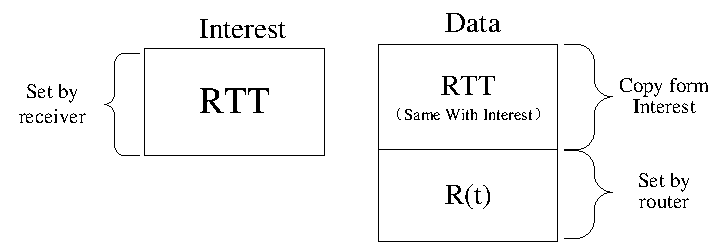
\includegraphics[width=3in]{header-ndn.pdf}
% where an .eps filename suffix will be assumed under latex,
% and a .pdf suffix will be assumed for pdflatex; or what has been declared
% via \DeclareGraphicsExtensions.
\centering
\caption{Explicit congestion notification header for Interest and Data}
\label{fig-header}
\end{figure}
It is critical to calculate the \emph{R(t)} for each router. Suppose we know how many flows going through this link, and we want to share the bandwidth with all the flows, \emph{R(t)} is possible to calculate as follow:
\begin{equation}
R(t)=\frac{C}{Flow_{num}*Size_{d}}
\end{equation}

$\emph{Size}_{\emph{d}}$ is the size of incoming Data. $\emph{Flow}_{\emph{num}}$ is the flow number on the link. Eq. 1 is the ideal situation. When the network condition changes, \emph{R(t)} should update. To make the update reasonable and let the system enter stable situation, Eq. 1 should evolve as:
%\begin{small}
\begin{equation}
R(t)=R(t-RTT_{avg})+\frac{\alpha(C-S(t))-\beta\frac{Q(t)}{RTT_{avg}}}{Flow_{num}*Size_{d}}
\end{equation}
%\end{small}

\emph{R(t)} is the Interest rate that the router assign to all flows at time \emph{t}. \emph{C} is the bandwidth of the link. \emph{S(t)} is the volume of coming back data in one time-unit. \emph{Q(t)} is the packets that occupied in the queue at time t.  $\alpha$ and $\beta$ is the parameters that influence the convergence and performance.  $\emph{RTT}_{\emph{avg}}$ is the average RTT of all the flows that go through this router. We set $\emph{RTT}_{\emph{avg}}$ as the rate updating interval.

The reason we define the R(t) is easy to understand. The available bandwidth and queue should be fairly share by all the flows, so the link resource is divided by the number of flow. If $\emph{(C-S(t))}>0$, there are more available bandwidth to be used and should increase the rate. Otherwise, the bandwidth has been over used and should reduce the sending rate. We assume that the packets occupied in the queue should always come to zero. If it is not zero, the rate will be reduced. And in every $\emph{RTT}_{\emph{avg}}$ the router should drain $\emph{Q(t)}/\emph{RTT}_{\emph{avg}}$ data. Because the R(t) is the Interest sending rate, and the available resource is supplied to the data, so we divide it by the size of data.

If the router want to make the system converse to stable more quickly, it can update the R(t) with shorter interval T $(0<T\leq\emph{RTT}_{\emph{avg}})$. Then  Eq. 2 becomes:
%\begin{small}
\begin{equation}
R(t)=R(t-T)+\frac{\frac{T}{RTT_{avg}}\ast(\alpha(C-S(t))-\beta\frac{Q(t)}{RTT_{avg}})}{Flow_{num}*Size_{d}}
\end{equation}
%\end{small}

Using the prefix of the interest name to estimate how many flows going through the router will add complexity to the router. In\cite{RCP}, it has been proved that the processor-fair resource allocated way can estimate the flow number by the each flow's sending rate. Processor-fair means the routers fairly give the link bandwidth and queue resource to all flows this link. So we also use process-fair way to calculate how many flows going through this link:
%\begin{small}
\begin{equation}
Flow_{num}=\frac{C}{R(t-RTT_{avg})\ast{Size_{d}}}
\end{equation}
%\end{small}
As we set every flow share the link bandwidth equally, and every flow's rate is the same, it is reasonable to use Eq. 4 to estimate the number of flows. In Sec. \uppercase\expandafter{\romannumeral 5}, we will prove that the estimation is correctly, and can reflect the change of the flows.
Joining Eq.3 and Eq.4, then the equation becomes:
%\begin{scriptsize}
\begin{equation}
R(t)=R(t-T)[1+\frac{\frac{T}{RTT_{avg}}\ast(\alpha(C-S(t))-\beta\frac{Q(t)}{RTT_{avg}})}{C}]
\end{equation}
%\end{scriptsize}
Many factors may influence the size of Data in NDN, such as the different MTU of different link layer. So it will be very difficult to exactly measure the size of data. When we need to use the size of Data to test the the accuracy of the flow number estimation, we have to use the historical information to estimate the size of Data. From Eq. 5 we can find that, R(t) do not need to measure the flow number directly and the size of Data. That will greatly simplify the router's calculating process.
\subsection{Smart adaptive forwarding}
In this paper we just use the SDN-style way to control the forwarding process, not the route calculating process. The route algorithm in NDN is still on active research, and it is still un-complete. But from the algorithm proposed by now, we can see that the NDN route algorithm is different from TCP/IP\cite{ndnroute}. Traditional route protocol such as OSPF and RIP just have one single path for each destination. But in NDN, a data may place on different places, so there may be several paths to get a data. And even the data from the same provider may have different available paths. So in this paper, we assume the receivers have several paths to get a data, and the routers have known every hop of different paths. The SDN-style adaptive forwarding mechanism we proposed just has relationship with the choosing of forwarding interfaces from different paths.

Every router sends its own sending rate, the transmit delay and the bandwidth of the next hop to the controller at the interval of $\emph{RTT}_{\emph{avg}}$. After several $\emph{RTT}_{\emph{avg}}$, the controller can know every router's sending rate and the transmit delay of every hop. We call the information as forwarding-assistant information. The network��s route information can also be stored in the controller. By the forwarding-assistant information and route information, we can calculate the best forwarding strategy. The forwarding-assistant and route information stored in the controller is showing in Fig.\ref{fig-assistant-information}.

\begin{figure}[t]
\centering
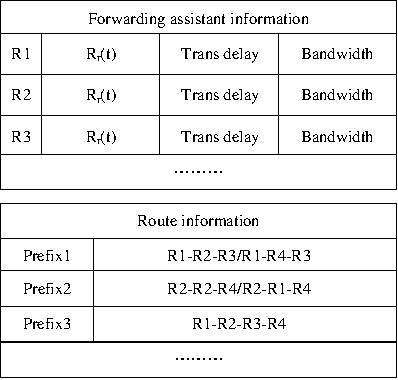
\includegraphics[width=2.5in]{forwarding-assistant-information.pdf}
% where an .eps filename suffix will be assumed under latex,
% and a .pdf suffix will be assumed for pdflatex; or what has been declared
% via \DeclareGraphicsExtensions.
\centering
\caption{Forwarding assistant and route information stored in the controller}
\label{fig-assistant-information}
\end{figure}


Using the rate Interest sending mechanism proposed above, the FCT of each flow is:
%\begin{footnotesize}
\begin{equation}
FCT=\frac{Size_{f}}{Size_{d}\ast{R_{b}}}+RTT
\end{equation}
%\end{footnotesize}
$\emph{Size}_{\emph{f}}$ is the size of the flow. $R_{b}$ is the path's bottleneck Interest sending rate. $R_{b}$ can be easily calculated by the forwarding-assistance and route information. Eq. 6 means that the FCT is the time that the flow going through the bottleneck plus the RTT of this flow. The RTT of this flow can be calculated by the forwarding-assistant information.
When a new flow enter, and it has serval paths to choose. We suppose it choose path j, then this flow's FCT on path j should be:
%\begin{footnotesize}
\begin{equation}
FCT_{i,j}=\frac{Size_{f}}{Size_{d}\ast{R^{'}_{b}}}+RTT_j
\end{equation}
%\end{footnotesize}
Where $RTT_j$ is the RTT if flow i choose path j and $R^{'}_{bottleneck}$ is the new bottleneck rate on path j.
%\begin{footnotesize}
\begin{equation}
R^{'}_{b}=\frac{C}{Flow_{num}+1}
=\frac{C}{C/(R_{b}\ast{Size_{d}})+1}
\end{equation}
%\end{footnotesize}
For simplify, we set the value of $Size_{data}$ and $Size_{flow}$ as fixed values. We suppose $Size_{data} =Size_{flow}$. So Eq. (7) becomes:
%\begin{footnotesize}
\begin{equation}
FCT_{i,j}=\frac{C/(R_{b}*Size_{d})+1}{C}+RTT_j
\end{equation}
%\end{footnotesize}
Our design goal is to minimum the Total Flow Complete Time (TFCT) in the network. TFCT is the sum of all the flows' complete time. To achieve our goal we define the objective of the smart forwarding as:
%\begin{footnotesize}
\begin{equation}\begin{aligned}
& \min &&  \sum_{i=0}^{n} FCT_i \\
& \text{s.t.}  && \text{path } j \text{ is available};\\
&              && \forall i, P_i \in \{0,1\};\\
&              && \max \min  R_i \enspace .
\end{aligned}
\end{equation}
%\end{footnotesize}
$P_i$ is the number of choosing path for $Flow_i$. $P_i \in \{0,1\}$ means there at most 1 path for $Flow_i$. $max \ min \ R_i$ means $Flow_{i}$'s Interest sending rate should be max . The reason we set $max \ min \ R_i$ is to achieve fairness of different flows.  If we do not set $max \ min \ R_i$, some flow may choose a min R to achieve minimum the TFCT, and that will influence this flow's FCT. Sacrificing oneself to achieve the goal of minimum TFCT is unfair.

Routers send the updated forwarding-assistance and route information to the controller at the interval of $\emph{RTT}_{\emph{avg}}$. The router send back smart forwarding decision for each flow when it receives the router's updating information. The smart forwarding decision is based on the unit of flow, not the unit of each packet. So the overhead introduced by the SDN-style help is very limited compared with the whole volume that go through the router. To timely reflect the change of network information to the controller, routers can change the sending interval, and that will raise the overhead. But the balance between the overhead and the accuracy of updating information can be adaptively controlled.

\subsection{Stability analysis}
The parameters $\alpha$ and $\beta$ influence the stability and convergence of the system. As Eq. 2 shows, $\alpha$ influences how the bandwidth is use. If $\alpha$ is large then bandwidth will be occupied quickly. $\beta$ influences how quickly that the packets in the queue can be drained. Obviously that large $\alpha$ and $\beta$ can help the system to use the resource quickly. But large $\alpha$ and $\beta$ will make the system becomes unstable, as the network is difficult to convergence.

To choose suitable $\alpha$ and $\beta$ that make the system stable, we test under what $\alpha$ and $\beta$ , the flow number can be estimated accurately. Once the flow number of the network can be accurately estimated, the Interest sending rate \emph{R(t)} can also be estimated accurately, then the system will enter stable stage. So we choose the accuracy of estimating flow number as the stability evaluation criteria.

At first there are 10 flows in the network, and we test wether the flow number can accurately be estimated under different value of $\alpha$ and $\beta$ . Fig. \ref{fig-ab}. shows that under such values the flow number can be accurately estimated. Fig. \ref{fig-abwrong}. shows that under these values the estimated flow number change heavily which means that the system is not stable. From Fig. \ref{fig-ab}., we can find (0.2,1.5) is the most suitable value to estimate the flow number. Under this value, we test wether the system is still stable when the system changes. We set 5,10,15 and 20 flows in the network respectively. Fig. \ref{fig-abflownum}. shows that under different situation the flow number can also be accurately estimated when $\alpha=0.2 \beta=1.5$. That means a fit value of $\alpha$ and $\beta$ can make the system enter stable stage even when the system's situation changes.

From Fig. \ref{fig-abwrong}., we find that when $\alpha$ close to 0.5, the system becomes unstable, and when it is larger than 0.5, the system becomes even more unstable. We think it is because large $\alpha$ make the system react too radically to increase \emph{R(t)}(when \emph{(C-S(t))}$>$0) or decrease \emph{R(t)}(when \emph{(C-S(t))}$<$0)(as Eq. 5 shows). Radical reaction will make the system difficult to converge. From Fig. \ref{fig-ab}., we find that when $\alpha$ $<$0.2, the system will take longer time to accurately estimate the flow number. It is because small $\alpha$ makes the system increase or decrease \emph{R(t)} conservatively, and that will result in longer time to convergence. When $\beta$ smaller than 1.5, although the system can be stable, the estimated flow number is not accurate compared with when $\beta$ = 1.5. It is because small $\beta$ can not drain the packets in the queue quickly enough. And that will result in inaccurate \emph{R(t)} and flow number.

The key point of the stability analysis is that, for $\alpha$ and $\beta$ we can choose a fit value to make the system stable. Even when the system change, such as the flow number, RTT and bandwidth, the fit value can also make the system keep stable. Although now we can not prove the best value by theory, it is possible to choose a suitable value by experimental test. In our simulation, we set $\alpha$ = 0.2 and $\beta$ =1.5, according the analysis above.
\begin{figure}[t]
\centering
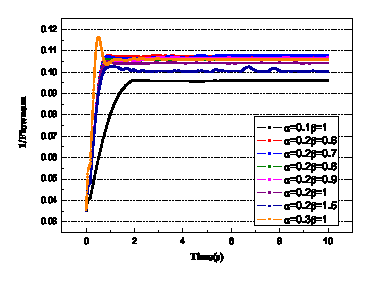
\includegraphics[width=2.5in]{ab-pic-cut.eps}
% where an .eps filename suffix will be assumed under latex,
% and a .pdf suffix will be assumed for pdflatex; or what has been declared
% via \DeclareGraphicsExtensions.
\centering
\caption{Under such $\alpha$ and $\beta$ the flow number can be accurately estimated}
\label{fig-ab}
\end{figure}
\begin{figure}[t]
\centering
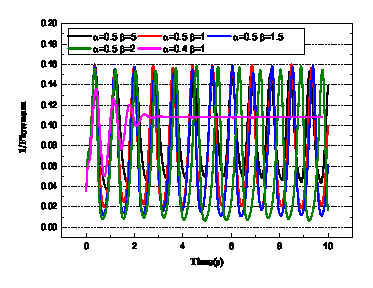
\includegraphics[width=2.5in]{abwrong-pic-cut.eps}
% where an .eps filename suffix will be assumed under latex,
% and a .pdf suffix will be assumed for pdflatex; or what has been declared
% via \DeclareGraphicsExtensions.
\centering
\caption{Under such $\alpha$ and $\beta$ the flow number can not be accurately estimated}
\label{fig-abwrong}
\end{figure}
\begin{figure}[t]
\centering
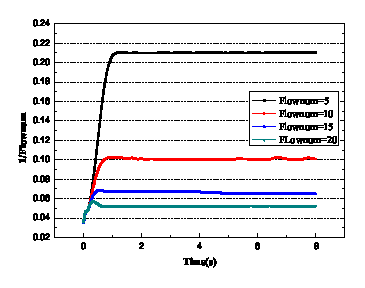
\includegraphics[width=2.5in]{abflownum-pic-cut.eps}
% where an .eps filename suffix will be assumed under latex,
% and a .pdf suffix will be assumed for pdflatex; or what has been declared
% via \DeclareGraphicsExtensions.
\centering
\caption{Stable $\alpha$ and $\beta$ can make the network stable even when network situation changes}
\label{fig-abflownum}
\end{figure}
\section{Simulation}
\subsection{Simulation setup}
In this section, we study the performance of the smart explicitness congestion notification mechanism for NDN we proposed using ndnSim. NdnSim is a NDN simulation environment developing under ns-3\cite{ndnsimnet} \cite{ndnsim}.

Fig.\ref{fig-topology}. shows the network topology we use in the simulation. There are two topologies we use. One is bottleneck topology and the other is mesh topology. In both network topologies, there are many consumers who send Interest into network and can get responding Data from the producer. The number of consumers is between [1,100], and each consumer requests Data with a same prefix (means they are a same flow). In the mesh network, consumers can get Data from three paths and each path's bottleneck bandwidth is different. Each link��s capacity varies form [30,200]Mbps and the propagation delay of each hop is 10ms. The buffer in each node is production of RTT and bandwidth. In the following figures, the bandwidth means the bottleneck��s bandwidth.

We set the value of �� and �� as 0.2 and 1.5. We compare our smart-ECN with ICP and ICP-shape. ICP is a TCP-style Interest control protocol in NDN. The Interest sending window is passively changed according the RTT and loss of Data, following the AIMD principle\cite{ICP}. ICP-shape also follows the AIMD principle but it discards the Interest instead Data when the routers sense congestion\cite{improveshape}. ICP-shape also sends NACK back to receiver if an Interest is shaped. NACK is a feedback information used to inform that the Interest has been discarded or there are not Data to response the Interest. The consumer should retransmit the same Interest when it receive a NACK.

Our simulation include three parts. In the first part we evaluate the flow number estimating process, which we propose in Eq.4. In the second part, we will evaluate the ECN Interest sending rate mechanism using the bottleneck network topology. At last we will estimate the smart forwarding mechanism using the mesh network topology. The simulation result shows the number flows can be estimated accurately. Compared with ICP and ICP-shape, ECN Interest sending rate mechanism performance better in link utilization, packets dropping and flow complete time. Our smart forwarding mechanism has better TFCT compared with adaptive forwarding mechanism.
\begin{figure}[t]
\centering
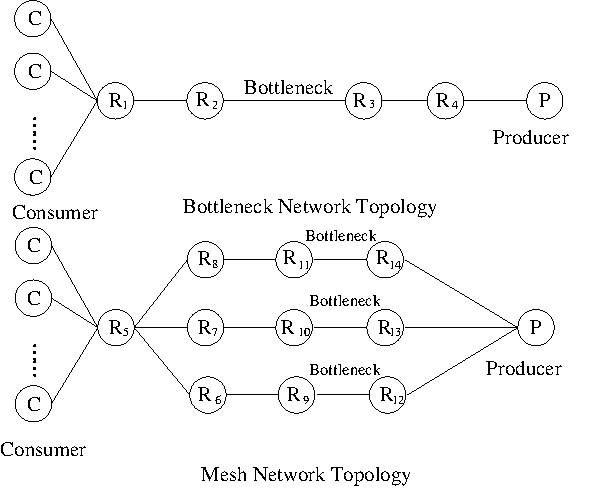
\includegraphics[width=3in]{topology.pdf}
% where an .eps filename suffix will be assumed under latex,
% and a .pdf suffix will be assumed for pdflatex; or what has been declared
% via \DeclareGraphicsExtensions.
\centering
\caption{The tow network topologies using in simulation}
\label{fig-topology}
\end{figure}
\subsection{The estimated flow number}
By Eq. 4 $Flow_{num}=\frac{C}{R(t-RTT_{avg})\ast{Size_{d}}}$, the flow number of the link can be estimated by the rate of this link. The size of data can be estimated as the average size of the data going through. Under the bottleneck network topology, at t=0, 10flows start. At t=10 more 10 flows start. And at t=20, 10 flows finish, remaining just 10 flows. From Fig.\ref{fig-flownum}. we can see that the flow number can be accurately estimated. Even when the flow number changes, the estimation can also converge.
\begin{figure}[t]
\centering
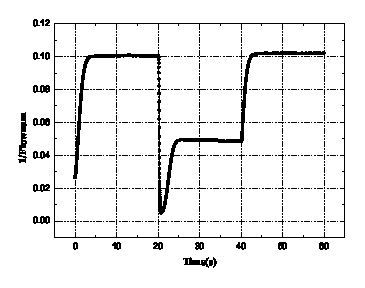
\includegraphics[width=2.5in]{flownum-pic-cut.eps}
% where an .eps filename suffix will be assumed under latex,
% and a .pdf suffix will be assumed for pdflatex; or what has been declared
% via \DeclareGraphicsExtensions.
\centering
\caption{The accuracy of estimated flow number}
\label{fig-flownum}
\end{figure}

\subsection{The performance of ECN Interest sending rate mechanism}

We use bottleneck topology to estimate the ECN Interest sending rate mechanism. The ECN Interest sending rate is calculated based on the principle that the whole bandwidth should be shared by the flows going through this link. The consumers send the Interest according the rate given by the bottleneck��s rate. Even when we change the bottleneck link's bandwidth, the bandwidth can be ultimately used, as the Fig.\ref{fig-linkuti}. shows. The ICP and ICP-shape use the TCP-style window control way. TCP-style window control way uses the timeout-principle to sense the congestion, and once timeout, it cut the interest window to half.  TCP-style window control also use the slow start way to send the interest. These will waste a lot of bandwidth.
\begin{figure}[t]
\centering
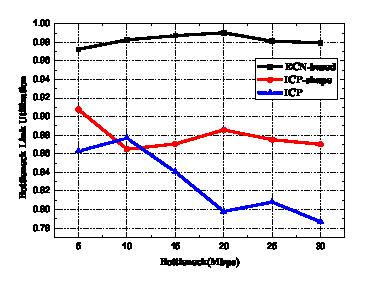
\includegraphics[width=2.5in]{utilization-pic-cut.eps}
% where an .eps filename suffix will be assumed under latex,
% and a .pdf suffix will be assumed for pdflatex; or what has been declared
% via \DeclareGraphicsExtensions.
\centering
\caption{Bottleneck link utilization compared with ICP when change the bottleneck bandwidth}
\label{fig-linkuti}
\end{figure}

Because the rate we calculate make sure that the rate can not overflow the bandwidth, almost no packets(no matter interest or data) drop in ECN interest sending rate mechanism, as the Fig.\ref{fig-drop}. shows. As the ICP-shape shapes the interest before congestion happens, it can reduce the data needed to be dropped because of congestion. But as the delay of sending back and the difficulty of estimating the congestion, there are still possible dropping data.
\begin{figure}[t]
\centering
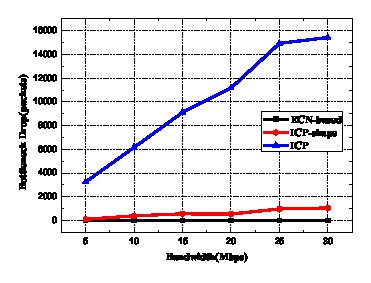
\includegraphics[width=2.5in]{drop-pic-cut.eps}
% where an .eps filename suffix will be assumed under latex,
% and a .pdf suffix will be assumed for pdflatex; or what has been declared
% via \DeclareGraphicsExtensions.
\centering
\caption{Bottleneck dropping packets compared with ICP when change the bottleneck bandwidth}
\label{fig-drop}
\end{figure}

As the Eq. 5 shows, the packets in the queue should do the utmost to be drained. This principle makes sure that in stable environment, the packets in the queue are always close to 0, as Fig.\ref{fig-queue}. shows. If there are more flows going through it, more packets will be queued, but as the rate decreases, the queuing packets will be drained after several RTTs. In ICP or ICP-shape, the packets in the queue is large. To use the bandwidth effectively, the receivers always try to make the Interest window large until the Data fills up the queue and drop the data. So for ICP and ICP-shape, the packets in the queue is much large than the ECN Interest sending rate mechanism.
\begin{figure}[t]
\centering
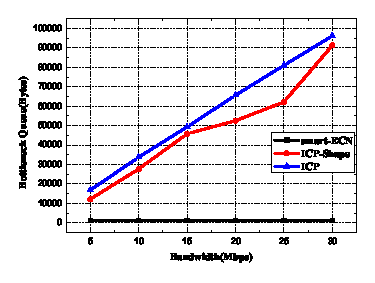
\includegraphics[width=2.5in]{queu-pic-cut.eps}
% where an .eps filename suffix will be assumed under latex,
% and a .pdf suffix will be assumed for pdflatex; or what has been declared
% via \DeclareGraphicsExtensions.
\centering
\caption{ Bottleneck queuing packets compared with ICP when change the bottleneck bandwidth}
\label{fig-queue}
\end{figure}

Fig.\ref{fig-fct}. shows the FCT of different flows. Flow complete time in NDN is defined as the time from when receiver send the first Interest until the receiver receive the last Data of the flow. As Fig.\ref{fig-linkuti}. shows, the ECN Interest sending rate mechanism��s link utilization is much higher than ICP. So no matter short flows or long flows, its FCT is much better than ICP. ECN Interest sending rate mechanism fairly applies bandwidth resource to all the flows, so even if the short flow can get fair bandwidth resource. In ICP short flows get less bandwidth resource compared with long flows, because the slow start principle.
\begin{figure}[t]
\centering
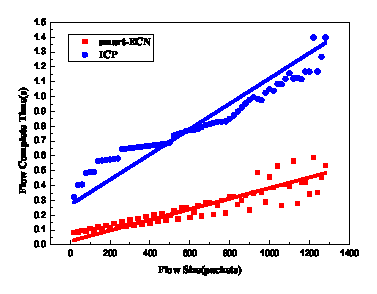
\includegraphics[width=2.5in]{fct-cut.eps}
% where an .eps filename suffix will be assumed under latex,
% and a .pdf suffix will be assumed for pdflatex; or what has been declared
% via \DeclareGraphicsExtensions.
\centering
\caption{ Flow Complete Time}
\label{fig-fct}
\end{figure}
\subsection{Flow complete time compared with ICP}


We demonstrate the effectiveness of smart adaptive forwarding mechanism using mesh network topology. Using the SDN control information, the smart adaptive forwarding mechanism can choose a network-wide best path. The adaptive mechanism chooses the best forwarding interface just by the next hop��s link information. As the next hop link information can not reflect the whole path��s information, the adaptive mechanism will sometimes choose a wrong path whose later link is shared by far more flows. The without-adaptive mechanism choose the path just by the route information, similar with TCP/IP.  The without-adaptive mechanism can not change the forwarding interface according the network condition. It is possible to choose a path that all the flows going through it, and that will greatly increase all the flows' complete time. As Fig.\ref{fig-tfct}. shows, under different total bandwidth, the smart adaptive forwarding's TFCT is much better than other two mechanisms.
\begin{figure}[t]
\centering
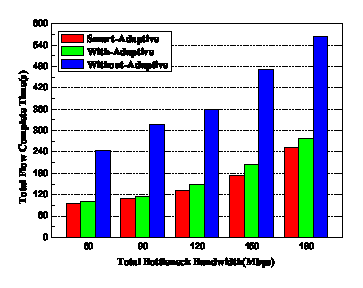
\includegraphics[width=2.5in]{adaptive-pic-cut.eps}
% where an .eps filename suffix will be assumed under latex,
% and a .pdf suffix will be assumed for pdflatex; or what has been declared
% via \DeclareGraphicsExtensions.
\centering
\caption{Total flow complete time compared with forwarding mechanisms}
\label{fig-tfct}
\end{figure}

\section{Related work}
Some transport mechanisms have been proposed for NDN. Most of them is TCP-style. Some researchers use NDN's features, such as the NACK, to improve the TCP-style mechanism.

Receiver driven TCP-style. Different with TCP/IP��s push principle, NDN is a pull-way architecture. So it is the receivers no longer the senders who dominant the traffic of network. Most of NDN transport mechanisms now proposed is receiver-driven. Receivers adjust its Interest sending window according to the RTT of the coming back Data, using the AIMD and slow start principle\cite{TCP}, similar with traditional network. Contug\cite{Contug} is the first TCP-style receiver-driven mechanism in NDN, following the basic principle in TCP. It just changes the congestion-controller from sender to receiver.  In\cite{Flow}, Sara, etc. use the prefix of the name to separate the traffic into different flows. Each flow uses TCP-like mechanism to control the congestion. Routers fairly share the bandwidth to each flow, and using optimal buffer algorithm to improve the performance. In NDN, in-network cache is available. T content can be get from different providers or routers. Different locations of content may result in multipath in transport layer. In \cite{Multipath}, Givonaan, etc. deal with the multipath problem in NDN, using similar way as the MTCP.

Interest NACK. In NDN the Interest is much shorter than Data. Intuitively, it is much more ��resource-saving�� if we drop Interest instead of Data when congestion happens. In HR-ICP\cite{shape}, routers shape the Interest hop-by-hop to deal with or avoid congestion. Each router shapes Interest just by itself, according the bandwidth it can supply to coming Data. In \cite{improveshape} Wang, etc. improve the Interest shaping mechanism. Once an Interest is shaped, router sends NACK Interest back to the receiver to inform that congestion has happened. The NACK sending back to the receiver is useful information to inform the receiver that congestion happens. But it is still implicit information, does not inform the degree of congestion. The receiver simply cut half of the Interest sending window when it receives the congestion signal. That will reduce the link utilization as in TCP. And the shaping mechanism, no matter Interest or Data will cause retransmit. Retransmit will increase the flow complete time.

To fit the pull principle of NDN, all of these above mechanisms use the receiver to deal with the congestion. But they still follow the TCP's slow start and AIMD implicit congestion principle, such as RTT and time-out packet loss. They also have the low utilization and unfair problems, similar with TCP\cite{NDNanalysis}.

\section{Conclusion}
In conclusion, we propose a ECN congestion control and a smart forwarding mechanism in NDN. Datas carry the ECN information to receivers. Receivers use ECN information to adjust its Interest sending rate. Under smart forwarding mechanism, routers choose a best forwarding interface using the SDN controller's network-view information. The ECN congestion control mechanism can ultimately use the link utilization and reduce the dropping packets. By joining the smart forwarding and ECN transport mechanism, the whole network resource can be effective used and total flow complete time can be reduced.

The future work will be focused on the theory proven of the system stability. In NDN, as the in-network cache, the Data's providers can be changed. That will influence the ECN information coming back the receiver and the RTT. We also want to analysis what would happen on such situation and how to make effective resolution for this.
% conference papers do not normally have an appendix


% use section* for acknowledgement
%\section*{Acknowledgment}

% trigger a \newpage just before the given reference
% number - used to balance the columns on the last page
% adjust value as needed - may need to be readjusted if
% the document is modified later
%\IEEEtriggeratref{8}
% The "triggered" command can be changed if desired:
%\IEEEtriggercmd{\enlargethispage{-5in}}

% references section

% can use a bibliography generated by BibTeX as a .bbl file
% BibTeX documentation can be easily obtained at:
% http://www.ctan.org/tex-archive/biblio/bibtex/contrib/doc/
% The IEEEtran BibTeX style support page is at:
% http://www.michaelshell.org/tex/ieeetran/bibtex/
%\bibliographystyle{IEEEtran}
% argument is your BibTeX string definitions and bibliography database(s)
%\bibliography{IEEEabrv,../bib/paper}
%
% <OR> manually copy in the resultant .bbl file
% set second argument of \begin to the number of references
% (used to reserve space for the reference number labels box)
\begin{thebibliography}{1}

\bibitem{NDN}
V. Jacobson, D. K. Smetters, J. D. Thornton, M. F. Plass, N. H. Briggs,
and R. L. Braynard, ``Networking named content," in Proceedings of ACM
CoNEXT, 2009.
\bibitem{ICP}
G. Carofiglio, M. Gallo, and L. Muscariello, ``ICP: Design and evaluation
of an interest control protocol for content-centric networking," in Proc.
1st IEEE Int��l Workshop on Emerging Design Choices in Name-Oriented
Networking, 2012.
\bibitem{Adaptive}
C. Yi, A. Afanasyev, L. Wang, B. Zhang, and L. Zhang, ``Adaptivd forwarding
in named data networking," in SIGCOMM Comput.Commun.Rev, 2012.
\bibitem{CCTCP}
L. Saino, C. Cocora, and G. Pavlou, ``CCTCP: A scalable receiver-driven
congestion control protocol for content centric networking," in Proc.IEEE ICC Int��l Conference, 2013.
\bibitem{shape}
N. Rozhnova and S. Fdida, ``An effective hop-by-hop interest shaping
mechanism for ccn communications," in Proc.1st IEEE Int��l Workshop on Emerging Design Choices in Name-Oriented Networking, 2012.
\bibitem{SDN}
A. Voellmy and J. Wang, ``Scalable software defined network controllers," in ACM SIGCOMM Computer Communication Review, 2012
\bibitem{XCP}
D. Katabi, M. Handley and C. Rohrs, ``Congestion control for high
bandwidth-delay product networks," in Proc.of ACM SIGCOMM,2002.
\bibitem{RCP}
N. Dukkipati, M. Kobayashi, R. Zhang-Shen, and N. McKeown, ``Processor
sharing flows in the internet," in IWQOS, 2006.
\bibitem{TCP}
V. Jacobson, ``Congestion avoidance and control," in SIGCOMM Comput.Commun.Rev, 1988.
\bibitem{selfish}
L. Qiu, Y. R. Yang, Y. Zhang, and S. Shenker, ``On selfish routing in internet-like environments," in Proc. of the ACM SIGCOMM,2003.
\bibitem{ndnroute}
R. Ahmed, and M. F. Bari, `` $\alpha$Route: A Name Based Routing Scheme for Information Centric Networks," in Proc. of IEEE INFOCOM 2013.
\bibitem{NDNanalysis}
S. Braun, M. Monti, M. Sifalakis and C. Tschudin, ``An empirical study of
receiver-based AIMD flow control strategies for CCN," in IEEE ICCCN,2013.
\bibitem{Flow}
S. Oueslati, J. Roberts, and N. Sbihi, ``Flow-aware Traffic Control for
a  Content -Centric Network," in IEEE INFOCOM, 2012.
\bibitem{Multipath}
G. Carofiglio, M. Gallo, and L. Muscariello, ``Multipath congestion control in content-centric networks," in IEEE INFOCOM, 2013.
\bibitem{Contug}
S. Arianfar, P. Nikander, L. Eggert, and J. Ott, ``Contug: A receiver driven transport protocol for content-centric networks," in IEEE ICNP 2010 (Poster session),2010.
\bibitem{improveshape}
Y. G. Wang, N. Rozhnova, A. Narayanan, D. Oran, and I. Rhee, ``An improved hop-by-hop interest shaper for congestion control in named data networking," in Proc. Of ACM SIGCOMM ICN, 2013.
\bibitem{ndnsimnet}
http://ndnsim.net/
\bibitem{ndnsim}
A. Afanasyev, I. Moiseenko, and L. Zhang, ``ndnSIM: NDN simulator for NS-3," in NDN, Technical Report NDN-0005, 2012.


\end{thebibliography}


% that's all folks
\end{document}


